The model's performance was evaluated using the MAE and RMSE metrics.
Table~\ref{tab:model_performance_comparison} shows a comparison between our model and the baseline, including the DCRNN~
\cite{DCRNN} and the STGM~\cite{LABLACK2023120281}.
The horizon is set to 1 hour (12 time steps).

NOTE: further experiments are in progress to get better comparisons to the baseline, like using other metrics and other
horizons.

\begin{figure}[htbp]
    \centering
    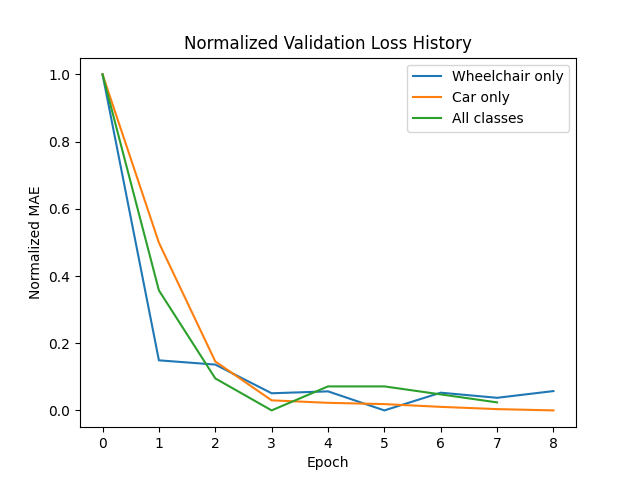
\includegraphics[width=0.5\textwidth]{images/normalized_val_losses}
    \caption{
        Plot of normalized validation losses during 3 trainings, one with only car data,
        one with only wheelchair data and one with both.
    }
    \label{fig:normalized_val_losses}
\end{figure}

\begin{table}[htbp]
    \caption{Model performance comparison on the METR-LA dataset, with~\cite{DCRNN},
        ~\cite{LABLACK2023120281}}
    \center
    \begin{tabular}{@{}llllll@{}}
        \toprule
        \textbf{Metric} & \textbf{STGM} & \textbf{DCRNN} & \multicolumn{3}{c}{\textbf{Adapted DCRNN}} \\
        & \textbf{Cars} & \textbf{Cars} & \textbf{Cars} & \textbf{Wheelchairs} & \textbf{All} \\
        \midrule
        MAE  & 3.60          & 3.23          & 2.67          & 0.08                 & 6.84         \\
        RMSE & 7.59          & 7.09          & 8.59          & 0.18                 & 14.8         \\
        \bottomrule
    \end{tabular}
    \label{tab:model_performance_comparison}
\end{table}